% Paul E. West and Sean T. Hayes
\documentclass[14pt,aspectratio=1610]{beamer}
% \documentclass[12pt,aspectratio=1610,handout]{beamer}
\usepackage{csu-theme}
\usepackage{tikz}
\usetikzlibrary{positioning}

\title{\Huge{} Basic Unix Commands}
\subtitle{CSCI 315: \textit{Data Structure Analysis}}
\author{Sean T. Hayes, Ph.D.}
\institute{Charleston Southern University}

%% Comment out date to use default (today)
% \date{January 14, 2025}
\subject{Data Structures}

\graphicspath{{../imgs/bash}}

\begin{document}

\begin{frame}
  \titlepage
\end{frame}


\section{Introduction}

\begin{frame}{Learning Outcomes}
\begin{itemize}
    \item Identify and use common Unix/Linux commands \\for file and directory management.
    \item Operate basic text editors in a Unix environment.
    \item Understand and apply file permissions and user/group management commands.
    \item Use input/output redirection and pipes to manipulate command-line data.
    \item Utilize regular expressions for pattern matching in file operations.
    \item Locate and interpret system and user information using Unix commands.
\end{itemize}
\end{frame}

%\begin{frame}{}
%\begin{itemize}
%\item Although modern Linux is equipped with a \textit{fancy schmancy} Graphical User Interface (GUI), 
%for system administrators (and *\textit{real}* programmers), shell is the best tool to handle everything.
%\item In GUI mode, you can activate our shell by opening a terminal window.
%\item The terminal window is your control panel for the system.
%\end{itemize}
%\end{frame}

% \begin{frame}{SSH over to Zion}
% \item<+-> SSH over to Zion:
% \begin{itemize}
% \item Alternatively, SSH (using \href{https://www.chiark.greenend.org.uk/~sgtatham/putty/}{PuTTY}) to Zion.
% \item Zion is a machine running on the CSU network.
% \item To SSH over:
% \begin{itemize}
% \item Linux: \lstinline{ssh -p 2222 coins.csuniv.edu}
% \item Windows: Download \href{https://www.chiark.greenend.org.uk/~sgtatham/putty/latest.html}{PuTTY} and enter coins.csuniv.edu with port 2222
% \item For either OS, use your CS CSU username and password.
% \end{itemize}
% \item All packages should be installed.
% \item Keep in mind that the system may go down from time to time.
% \end{itemize}
% \end{enumerate}
% \end{frame}

\section{Text Editors}

\begin{frame}{Choosing a Text Editor}
\begin{itemize}[<+->]
\item Take the time to choose a good text editor.
\begin{itemize}
\item You will be using it a lot. Investing the time to learn now will greatly pay off.
\end{itemize}
\item Linux has numerous choices.
\item Be aware that people become very passionate about which text editor is best.
\end{itemize}
\end{frame}

\begin{frame}{Vi, Vim, Neovim}
Lightweight with a high learning curve, but \textit{fast} once learned.
\begin{columns}[c]%
\column{0.45\textwidth}%
\begin{tabular}{c l}%
  \texttt{:q}  & to quite from vim\\
  \texttt{:wq} & to write change and quit\\
  \texttt{:q!} & to quit without saving\\
  \texttt{ESC} & to exit from editing mode\\
  \texttt{i}   & to insert\\
  \texttt{x}   & to delete a char\\
  \texttt{dd}  & to delete a line\\
  \texttt{/}   & to text search\\
\end{tabular}


\column{0.40\textwidth}
  \only<1>{
\includegraphics[width=1\textwidth]{vi-meme}}
  \only<2>{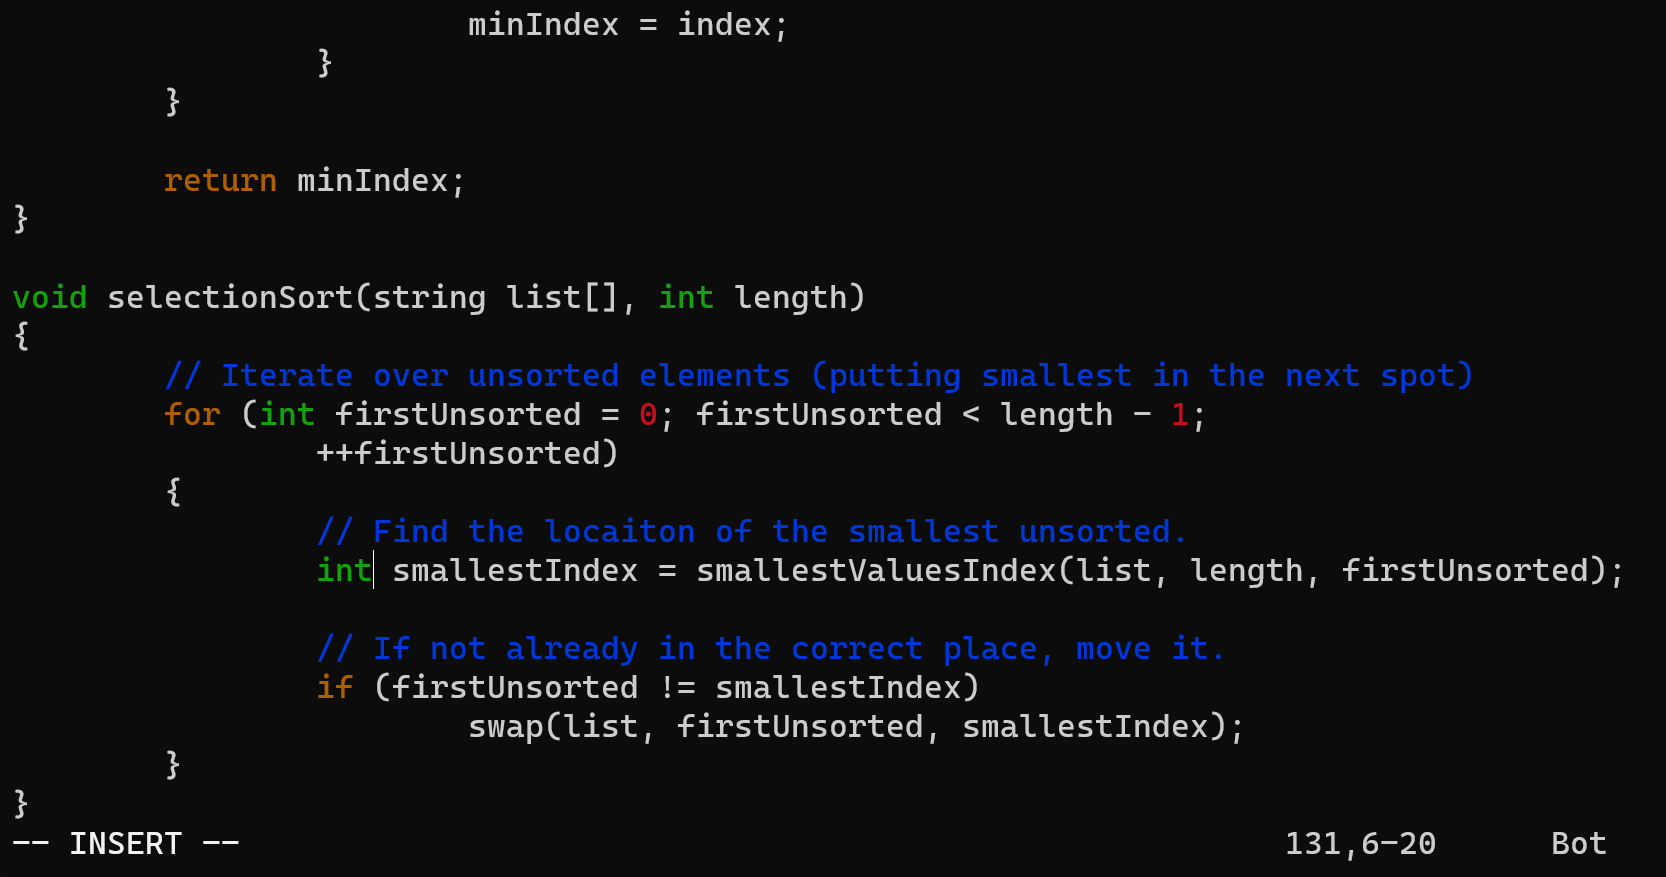
\includegraphics[width=1\textwidth]{vim}}
\end{columns}

\begin{itemize}
  \item The same on every machine.
  \item See the \href{https://vim.rtorr.com/}{cheat sheets}.
  \item Type \lstinline{vimtutor} in the terminal for an iterative tutorial.
\end{itemize}

\end{frame}

\begin{frame}{Emacs (Editor MACroS)}
\begin{columns}
\column{0.6\textwidth}
\begin{itemize}
\item Lots of features --- tons of capabilities
\item LISP
\item Your hand may be warped from all the hotkeys.
\item Not always the same on every machine.
\end{itemize}
\column{0.4\textwidth}

\includegraphics[width=1\textwidth]{emacs-meme}
\end{columns}
\end{frame}

\begin{frame}{nano}
\begin{columns}
\column{0.4\textwidth}
  \begin{itemize}
  \item Simple! The same on every machine.
  \item The commands are at the bottom of your screen.
    \begin{itemize}
    \item
      \texttt{\textbf{\^}} stands for \texttt{Ctrl}.
    \item
      \texttt{Ctrl} + \texttt{G} displays the help screen.
    \end{itemize}
  \end{itemize}
\column{0.6\textwidth}
  \only<1>{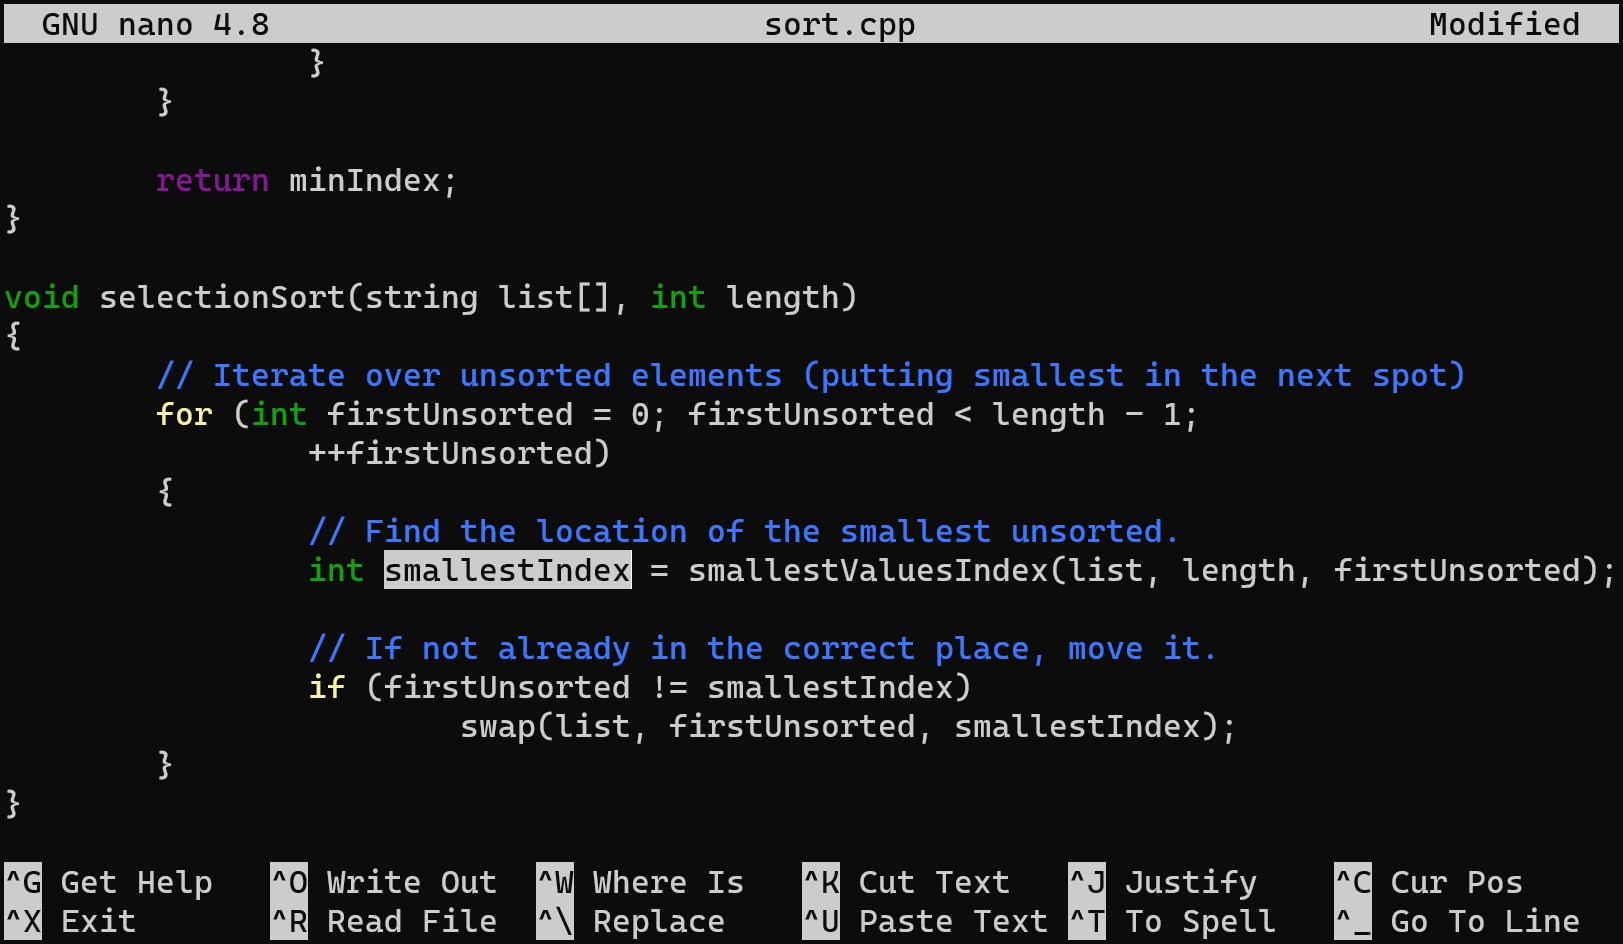
\includegraphics[width=1\textwidth]{nano}}
  \only<2>{\centerline{
\includegraphics[width=0.9\textwidth]{nano-meme}}}
\end{columns}
\end{frame}

\begin{frame}{Graphical Text Editors}
\begin{tabularx}{1\textwidth}{c X}
  \href{https://code.visualstudio.com/}{VS Code} & Microsoft's very popular open-source code editor, customizable, extensible.\\
  \href{https://vscodium.com/}{VSCodium} & Free/Libre Open Source VS Code\\
  gVim & graphical Vim\\
  Xemacs & graphical Emacs\\
  gedit & like MS WordPad/Notepad\\
  Sublime Text & newer, very powerful (unlimited free trial)\\
  Kate & KDE text editor\\
  Tea & Minimal Qt text editor\\
  Jed & Very basic.  Essentially nano++\\
\end{tabularx}
\end{frame}

\section{Directory Operations}
% \subsection{}
\begin{frame} {\texttt{\textbf{ls}} -- List files and directories.}
\lstinline{ls} displays a list of files in the current working directory, like
\lstinline{dir} in DOS.
\vspace{1em}

\begin{tabular}{l l}
  \lstinline{-a} & Display hidden (start with a `\lstinline{.}') files.\\
  \lstinline{-A} & Do not display `\lstinline{.}' and `\lstinline{..}'.\\
     & `\lstinline{.}'  means current directory.\\
     & `\lstinline{..}' means upper layer directory.\\
  \lstinline{-l} & Display file lists with long format.\\
  \lstinline{-s} & Display file size.\\
  \lstinline{-h} & Display sizes in a more human readable format.\\
\end{tabular}
\end{frame}

\begin{frame}{\texttt{\textbf{cd}} -- Change the working directory.}
Usage: cd \lstinline{DIRECTORY}\\\vspace{1em}

\begin{tabular}{l l}
  \lstinline{cd /usr/bin} & Change the directory to \lstinline{/usr/bin}.\\
  \lstinline{cd ..}       & Change to the parent directory. \\
  \lstinline{cd /}        & Change to the root directory. \\
  \lstinline{cd ~}        & Change to the user's home directory.\\
\end{tabular}
\end{frame}


\begin{frame}{\texttt{\textbf{mkdir}} -- Making Directories}
  \lstinline{mkdir DIRECTORY} -- Create the DIRECTORY(ies) that do not already exist.
  \begin{tabularx}{1\textwidth}{l X}
    \lstinline{mkdir temp}            & Make a directory named \lstinline{temp}.\\
    \lstinline{mkdir temp2}           & Make a directory named \lstinline{temp2}\\
    \lstinline{mkdir temp/insideTemp} & Make \lstinline{insideTemp} directory within \lstinline{temp}. \\
  \end{tabularx}\\\vspace{1em}
\end{frame}

\begin{frame}{\texttt{\textbf{rmdir}}/\texttt{\textbf{rm}} -- Removing Directories}
\lstinline{rmdir DIRECTORY} -- Remove \textit{empty} DIRECTORY(ies).
  \begin{tabularx}{1\textwidth}{l X}
    \lstinline{rmdir temp}            & Remove a directory named \lstinline{temp}.\\
    \lstinline{rmdir temp2}           & Remove a directory named \lstinline{temp2}\\
    \lstinline{rmdir temp/insideTemp} & Remove the \lstinline{insideTemp} directory that is within \lstinline{temp}. \\
  \end{tabularx}\\\vspace{1em}

\lstinline{rm -r DIRECTORY} -- Remove directories and their contents recursively.

\end{frame}

\begin{frame}{Directory Usage}
\begin{itemize}
\item Any command that accepts a file or folder as a parameter assumes that the file is in the \emph{present working directory} (PWD) unless told otherwise.
\item Use relative or absolute paths to indicate where a file is.
\item Absolute paths start with a \lstinline{/} and the path begins from the highest level.
\item Relative paths NEVER start with a \lstinline{/} and are how to get to the file from the PWD.
\item \lstinline{..} is your parent directory, useful in relative paths
\end{itemize}
\end{frame}

\section{File Operations}

%\begin{frame}{Creating a file with cat}
%cat is a command we will discuss later\\
%gedit, vi, and nano are text editors available in our Linux and can be used to create a file as well.
%\includegraphics[width=1.0\textwidth]{file-create.png} \\
%\end{frame}

\begin{frame}{\texttt{\textbf{cp}} -- Copy SOURCE to DEST.}
Usage: \lstinline{cp [OPTIONS] SOURCE DEST}

\begin{itemize}
  \item \lstinline{cp data1.txt data2.txt}
  \item \lstinline{cp data3.txt temp}

  \item Options:\\
  \begin{tabular}{l l}
    \lstinline{-i} & Ask before overwrite.\\
    \lstinline{-v} & Display copying process.\\
    \lstinline{-R} & Recursive copy, including sub-directories.\\
  \end{tabular}
  \item \lstinline{cp -R * backup} --  Copy all files in current directory into \lstinline{backup}.
\end{itemize}
\end{frame}

\begin{frame}{\texttt{\textbf{rm}} -- Remove the FILE(s).}

Usage: \lstinline{rm [OPTIONS] [FILES]}

\begin{itemize}
\item \lstinline{rm data1.txt}
\item \lstinline{rm *}

\item Options:\\
  \begin{tabular}{l l}
    \lstinline{-f} & Force remove files.\\
    \lstinline{-r} & Recursive remove files, including sub-directories.\\
    \lstinline{-v} & Display removing process.\\
  \end{tabular}

\item \lstinline{rm -f *.txt} -- Removes all files ending in .txt from the current directory.
\item \lstinline{rm -r *}  -- Removes all files and folders from the current directory.
\end{itemize}
\end{frame}


\begin{frame}{More File Operations}
\begin{itemize}
\item \lstinline{mv} -- Move files or rename a file.
\begin{itemize}
  \item \lstinline{mv data1.txt ..}
  \item \lstinline{mv data1.txt data4.txt}
\end{itemize}
\item<2-> \lstinline{pwd} -- Print (present) working directory.
\item<3-> \lstinline{file} -- Display file type.
\begin{itemize}
  \item \lstinline{file filename}
  \item \lstinline{file *}
\end{itemize}
\end{itemize}
\end{frame}

\begin{frame}{Even More File Operations}
\begin{itemize}
\item \lstinline{head} -- Displays the first 10 lines of each FILE.
\begin{itemize}
\item \lstinline{head data1.txt} shows first 10 lines of \lstinline{data1.txt}
\item \lstinline{head -20 data1.txt} shows first 20 lines
\end{itemize}
\item \lstinline{tail} -- Displays the last 10 lines of each FILE.
\begin{itemize}
\item \lstinline{tail data1.txt} shows last 10 lines of \lstinline{data1.txt}
\end{itemize}
\item \lstinline{wc} -- Displays line count, unique \textit{word count}, and total \textit{word count} for each FILE (and a total line if more than one FILE is specified).
\end{itemize}
\end{frame}

\begin{frame}{Yes, Even More File Operations}
\begin{itemize}
  \item \lstinline{find} -- Find files and directories (and perform operations on them).
    \begin{itemize}
      \item \lstinline{-name}	-- the filename you are looking for
      \item \lstinline{-print} -- output results
      \item \lstinline{find /usr -name config -print}\\%
        Displays where all the files named \lstinline{compress} are located.
    \end{itemize}
  \item<2-> \lstinline{grep} -- Search for PATTERNS in each FILE.
    \begin{itemize}
      \item Usage: \lstinline{grep [OPTIONS] PATTERNS [FILE].}
      % \item We may talk more about this command later.
    \end{itemize}
  \item<3-> \lstinline{ln} -- Create a link to TARGET with the name LINK\_NAME.
    \begin{itemize}
      \item Usage: \lstinline{ln [OPTIONS] TARGET LINK\_NAME}
      \item \lstinline{-s}  Create a symbolic link.
      \item \lstinline{ln -s target.txt newname.txt}
      \item More later on linking.
    \end{itemize}
\end{itemize}
\end{frame}

\section{Redirects}
\begin{frame}{Input/Output (I/O)}
  There are three standard input/output devices.

  \begin{tabular}{l l}
    \lstinline{stdin} & keyboard input\\
    \lstinline{stdout} & Monitor output\\
    \lstinline{stderr} & Error output device\\
  \end{tabular}\\[1em]

\center{}
\begin{tikzpicture}[
  node distance=3cm,
  box/.style={draw, very thick, fill=CSUcyan, text=black, minimum width=3cm, minimum height=1cm, text centered, align=center},
  arrow/.style={->, very thick, shorten >=1pt},
  label/.style={font=\ttfamily, inner sep=0pt}
]

  % Draw the central box
  \node[box] (process) {process \\ (your program)};

  % Draw "stdin" and its arrow pointing to the box
  \node[left of=process, label, anchor=east] (stdin) {stdin};
  \draw[arrow] (stdin) -- (process.west);

  % Draw "stdout" and its arrow leaving the box to the right
  \node[right of=process, label, anchor=west, yshift=-5mm] (stdout) {stdout};
  \draw[arrow] (process) -- (stdout);
  % \draw[arrow] (process.east) -- ++(2.5cm, 0.5cm) -- (stdout.west);

  % Draw "stderr" and its arrow leaving the box to the right
  \node[right of=process, label, anchor=west, yshift=5mm] (stderr) {stderr};
  \draw[arrow] (process) -- (stderr);

\end{tikzpicture}
\end{frame}

\begin{frame}{The Pipe Operator (\texttt{\textbf{|}})}
\begin{itemize}
\item Redirect output of one program to another.
\item For Example,\\
\lstinline{ls -al /etc | more}
\end{itemize}

\center{}
\begin{tikzpicture}[
  node distance=1.8cm,
  box/.style={draw, very thick, fill=CSUcyan, text=black, minimum width=2cm, minimum height=1cm, text centered, align=center},
  arrow/.style={->, very thick, shorten >=1pt},
  label/.style={font=\ttfamily\small, inner sep=0pt}
]
  % Draw the central box
  \node[box] (process) {ls};

  % Draw second process
  \node[right=4cm of process, box] (process2) {more};

  % Draw "stdin" and its arrow pointing to the box
  \node[left of=process, label, anchor=east] (stdin) {stdin};
  \draw[arrow] (stdin) -- (process.west);

  % Draw "stdout" and its arrow leaving the box to the right
  \node[right=0.5cm of process, label, anchor=west, yshift=-5mm] (stdout) {stdout};
  \node[left=0.5cm of process2, label, anchor=east, yshift=-5mm] (stdin2) {stdin};
  \draw[arrow] ([yshift=-2mm] process.east) -- ([yshift=-2mm] process2.west);

  % Draw "stderr" and its arrow leaving the box to the right
  \node[right of=process, label, anchor=west, yshift=5mm] (stderr) {stderr};
  \draw[arrow] (process) -- (stderr);

  % Draw "stdout2" and its arrow leaving the box to the right
  \node[right of=process2, label, anchor=west, yshift=-5mm] (stdout) {stdout};
  \draw[arrow] (process2) -- (stdout);

  % Draw "stderr2" and its arrow leaving the box to the right
  \node[right of=process2, label, anchor=west, yshift=5mm] (stderr) {stderr};
  \draw[arrow] (process2) -- (stderr);

\end{tikzpicture}


\begin{itemize}
\item This can continue on\textellipsis
\item What Data Structure does this look like?
\end{itemize}
\end{frame}

\begin{frame}{I/O Redirect to Files}
\begin{itemize}
\item Use \lstinline{<} and \lstinline{>} to redirect I/Os
\item \lstinline{cat > output.dat}
\item Use Ctrl-d to quit
\item \lstinline{cat >> output.dat}
\begin{itemize}
\item Append new output to the end of output.dat.
\end{itemize}
\item \lstinline{cat !> output.dat}
\begin{itemize}
\item Force overwrite output.dat.
\end{itemize}
\end{itemize}
\end{frame}

%\subsection{File Operations with Redirects}

\begin{frame}{Hey Look, Even \textit{More} File Operations!}
\begin{itemize}
\item \lstinline{more} -- Pause viewing output.
\begin{itemize}
  \item \lstinline{ls -al | more}
  \item \lstinline{more data1.txt}
\end{itemize}
\item \lstinline{less} -- Hmmm, what does less do?
  \begin{itemize}
    \item Type \lstinline{:q} to exit.
  \end{itemize}
\item \lstinline{cat} -- Display or \textit{concatenate} files.
\begin{itemize}
\item \lstinline{cat data1.txt | more}
\item \lstinline{cat data1.txt >> data2.txt}
\item \lstinline{cat data1.txt data2.txt >> data3.txt}
\end{itemize}
\item \lstinline{tac} -- Hmmm, what does \lstinline{tac} do?
\end{itemize}
\end{frame}

%\begin{frame}{Printing}
%\begin{itemize}
%\item lp
%\begin{itemize}
%\item prints the named files to the printer
%\item -d : specify the printer
%\item -n how many copies
%\end{itemize}
%\item lpstat
%\begin{itemize}
%\item displays the status of print jobs sent to any printer with the lp command
%\end{itemize}
%\item cancel
%\begin{itemize}
%\item removes all of the specified jobs from the printer queue
%\end{itemize}
%\end{itemize}
%\end{frame}

%\begin{frame}{Printing Continued}
%\begin{itemize}
%\item Some systems use different commands
%\item lpr
%\begin{itemize}
%\item for printing
%\item -P specify the printer
%\item -\# number of copies
%\item -m mail you when printing is done
%\end{itemize}
%\item lprm
%\begin{itemize}
%\item remove printing jobs
%\item -P specify the printer
%\end{itemize}
%\end{itemize}
%\end{frame}

\begin{frame}{Looking up how a command works.}
\begin{itemize}
\item The \lstinline{--help} argument displays how to use (almost) any command.
\begin{itemize}
  \item \lstinline{ls --help}
\end{itemize}
\item \lstinline{man} -- Display the \textit{manual} for a command.
\begin{itemize}
  \item \lstinline{man ls}
\end{itemize}
\item \lstinline{info} -- Displays the information about a command.
\begin{itemize}
  \item \lstinline{info ls}
\end{itemize}


\end{itemize}
\end{frame}

\section{RegEx}

\begin{frame}{Regular Expressions (RegEx)}
Sets of special characters that help you match a pattern.\\\vspace{0.5em}
\begin{tabularx}{1\textwidth}{c X}
  \hline
  \lstinline{*} & All possible combination(s)\\
    & \lstinline{des*} -- desk, desktop, description, \textellipsis\\
  \hline
  \lstinline{?} & Any single character\\
    & \lstinline{des?} -- desk, des9, \textellipsis\\
    & \lstinline{ls -al *.ps}\\
    & \lstinline{cat ??go}\\
    & \lstinline{more *a*b?}\\
  \hline
  \lstinline{[ ]} & Symbols in the square brackets\\
    & \lstinline{ls -al [ms]oon} displays files named: moon and soon\\
    & \lstinline{more [a-p]ount} displays contents of files named:\\
    & \hspace{3em} aount, bount, count, \textellipsis,  pount\\
\end{tabularx}
\end{frame}

%\begin{frame}{Advanced grep Operations}
%\begin{itemize}
%\item Global or Get Regular Expression and Print
%\item LEARN IT, it can save time
%\item grep -hilnvw pattern filename
%\item fgrep -hilnvwx string filename 
%\begin{itemize}
%\item Fixed grep, fast, only works with string
%\end{itemize}
%\item egrep -hilnvw pattern filename
%\begin{itemize}
%\item Extended grep, supports extended regular expression
%\end{itemize}
%\item Parameters:
%\begin{itemize}
%\item -n Print line number
%\item -w Restricts matching to whole words only
%\item -v displays all lines NOT matching
%\item -l displays a list of the files that contain the specified pattern, useful when filename has wildcards
%\item -x displays lines that are exactly equal to string
%\end{itemize}
%\end{itemize}
%\end{frame}
%
%\begin{frame}{Advanced grep Operations}
%\begin{itemize}
%\item cat > grepfile \\
%Well, you know it's your bedtime, \\
%So turn off the light, \\
%Say all your prayers and then, \\
%Oh you sleepy young heads dream of wonderful things, \\
%And you will be swimming through the sea \\
%\item grep the grepfile
%\item grep -wn the grepfile
%\item grep -v the grepfile
%\end{itemize}
%\end{frame}
%
%\begin{frame}{Advanced grep Operations}
%\begin{itemize}
%\item grep .nd grepfile
%\item grep $\hat{}$ .nd grepfile
%\item grep sw*.ng grepfile
%\item grep $[$A-D$]$ grepfile
%\item grep a. grepfile
%\end{itemize}
%\end{frame}

%\begin{frame}{Expressions}
%\begin{itemize}
%\item .	Matches any single character
%\item $[]$ Matches any single characters enclosed in brackets.
%\item If the first character after the $[$ is $\hat{}$ , then any character not enclosed in brackets is matched
%\item * May follow any character and denotes zero or more occurrences of the character that precedes it.
%\item $\hat{}$ Matches the beginning of a line only
%\item \$ Matches the end of a line only
%\end{itemize}
%\end{frame}

%\begin{frame}{Login and Logout}
%\begin{itemize}
%\item In GUI mode you can easily login and logout using mouse click
%\item In text mode, you have to use command to logout a system.
%\item After logout, do not power off the system!
%\end{itemize}
%\end{frame}

%\begin{frame}{Shutdown}
%\begin{itemize}
%\item time
%\begin{itemize}
%\item hh:mm - shutdown 10:45
%\item +m - shutdown +5
%\item now - shutdown now
%\end{itemize}
%\item warning message
%\begin{itemize}
%\item shutdown +5 "system will shutdown in 5 minutes"
%\end{itemize}
%\item r - reboot after shutdown
%\begin{itemize}
%\item shutdown -r now
%\item shutdown -r 23:50 \&
%\end{itemize}
%\item h - halt the system
%\begin{itemize}
%\item shutdown -h now
%\item After seeing "system halted", you can power off the system.
%\end{itemize}
%\item c - cancel shutdown command
%\begin{itemize}
%\item shutdown -c
%\end{itemize}
%\end{itemize}
%\end{frame}

%\begin{frame}{Reboot}
%\begin{itemize}
%\item -n - no sync before reboot
%\begin{itemize}
%\item sync - to flush buffer and write them back to disks
%\end{itemize}
%\item -f - force reboot
%\end{itemize}
%\end{frame}

%\begin{frame}{Man Page}
%\begin{itemize}
%\item The man command allows you to access the MANual pages for a UNIX command.
%\item To get additional help on any of the commands listed below, you can always type man name\_of\_command at the command prompt.
%\item Examples:\\
%man ls \\
%man cd
%\end{itemize}
%\end{frame}

\section{User Administration}
\begin{frame}{User-Management Tools}
\begin{itemize}
\item \lstinline{useradd} -- Adds a new user account to the system. Its options permit the sysadmin to specify the user's home directory and initial group or to create the user with the default home directory and group assignments.
\item \lstinline{useradd -D} -- Displays default settings for new users
\item \lstinline{useradd -G} -- Sets the system defaults for creating the users' home directory, account expiration date, default group, and command shell. See the specific options in \lstinline{man useradd}. Used without any arguments, it displays the defaults for the system. The default set of files for a user are found in \texttt{/etc/skel}.
\begin{itemize}
\item \lstinline{ls -al /etc/skel} -- will list the files with the defaults.
\end{itemize}
\end{itemize}
\end{frame}

\begin{frame}{User-Management Tools}
\begin{itemize}
\item \lstinline{userdel} -- Will completely remove a user's account (thereby eliminating that user's home directory and all files it contains).
\item \lstinline{passwd} -- Change a user's \textit{password}.
\item \lstinline{usermod} -- Changes several user attributes. The most commonly used arguments are -s to change the shell and -u to change the UID. No changes can be made while the user is logged in or running a process.
\item \lstinline{chsh} -- Changes the user's default shell. For Fedora, Debian, and others, the default shell is \texttt{/bin/bash}, known as the Bash (or Bourne Again Shell).
\end{itemize}
\end{frame}

\begin{frame}{}
\lstinline{useradd winnie -p gu1tarplayeR -s /bin/bash -u 507}
\begin{center}
  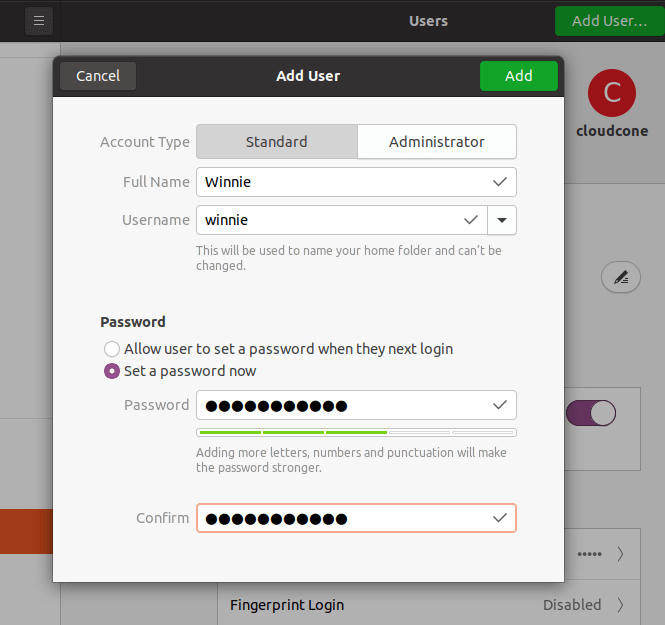
\includegraphics[width=0.5\textwidth]{useradd.png}%
\end{center}
\end{frame}

\begin{frame}[fragile]{}
  \begin{itemize}
  \item The password file is \texttt{/etc/passwd}, and it is the database file for all users on the system. The format of each line is as follows:\\
  \lstinline{username:password:uid:gid:gecos:homedir:shell}\\
  \item Example:\\
\begin{lstlisting}[basicstyle=\ttfamily\footnotesize, identifierstyle=\color{white}]
root:x:0:0:root:/root:/bin/bash
sshd:x:74:74:Privilege-separated SSH:/var/empty/sshd:/sbin/nologin
rpc:x:32:32:Portmapper RPC user:/:/sbin/nologin
rpcuser:x:29:29:RPC Service User:/var/lib/nfs:/sbin/nologin
nfsnobody:x:65534:65534:Anonymous NFS User:/var/lib/nfs:/sbin/nologin
mailnull:x:47:47::/var/spool/mqueue:/sbin/nologin
\end{lstlisting}
  \end{itemize}
\end{frame}

\begin{frame}{Group Hug}
  Groups establish relationships among users where they\\
  share a common set of permissions.
\begin{itemize}
\item<2-> All the groups are listed in \lstinline{/etc/group} file.
\item<3-> Group-Management Tools:
\begin{itemize}
\item Add a new group with the \lstinline{groupadd} command.\\
  \lstinline{groupadd www-data}
\item Change the group ownership of a file with the \lstinline{chgrp} command.\\
  \lstinline{chgrp www-data /srv/www}
\item Add the approved user to the group with \lstinline{usermod}.\\
  \lstinline{usermod -G www-data  shelley}
\item Make \texttt{shelley} the group administrator with \lstinline{gpasswd}, so that she can add new users to the group.\\
  \lstinline{gpasswd -A shelley}
\end{itemize}
%\item<4-> There is a GUI for group management as well.
\end{itemize}
\end{frame}

\begin{frame}{User Accounts}
\begin{itemize}
\item Usually, \texttt{/etc/passwd} holds user account information. Each user, regardless of type, will have a one-line entry of account information stored in this text file.
\item The superuser is known by the name \textit{root}.
\item User IDs and Group IDs
\item File Permissions:
  \begin{tabular}{@{$\bullet$ }ll}
    \lstinline{chgrp} & Changes the group ownership of a file.\\
    \lstinline{chown} & Changes the owner of a file.\\
    \lstinline{chmod} & Changes the access permissions of a file.\\
  \end{tabular}

\end{itemize}
\end{frame}

\begin{frame}[fragile]{File Permissions using \texttt{\textbf{chmod}}}
Try \lstinline{ls -l}.\\\vspace{0.5em}
{\footnotesize
\begin{lstlisting}[language={}]
- rwxr-xr-x joe acctg archive.sh
- rw-rw-r-- joe acctg orgchart.gif
- rw-rw-r-- joe acctg personnel.txt
- r--rw-r-- joe acctg public.html
d rwxr-xr-x joe acctg sales
- rw-r----- joe acctg topsecret.inf
- rwxr-xr-x joe acctg wordmatic
\end{lstlisting}}


\small
The first set of three letters after the file type describes the permissions the owner of the file has.\\\vspace{0.5em}

An \lstinline{r} in the first position means you are permitted to read the file.\\
A \lstinline{w} in the second position means you may write to or delete the file.\\
An \lstinline{x} in the third position means you may execute the file.\\\vspace{0.5em}

A hyphen represents a denied permission at its position.
\end{frame}

\begin{frame}{File Permissions using \texttt{\textbf{chmod}}}
The most succinct way to use \lstinline{chmod} is with numbers.  Each permission is assigned a value:\\
r = 4, w = 2, x = 1, Therefore,\\[0.5em]

\begin{tabular}{c l c}
\textbf{Value} & \textbf{Meaning} & \textbf{Binary}\\
0 & No permission    & \texttt{000} \\
1 & Execute only     & \texttt{001} \\
4 & Read only        & \texttt{100} \\
5 & Read \& Execute  & \texttt{101} \\
6 & Read \& Write    & \texttt{110} \\
7 & Full permission  & \texttt{111} \\
\end{tabular}
\end{frame}

\begin{frame}{Using \texttt{\textbf{chmod}}}
With \lstinline{chmod} you have three numbers: first for the owner, second for group, third for everyone else.

Let's look at some examples.\\
\begin{tabular}{| r  l |}
\hline
Before: & \lstinline{-rwxr-xr-x  archive.sh}\\
Command: & \lstinline[language=bash]{chmod 754 archive.sh} \\
After: & \lstinline{-rwxr-xr-- archive.sh} \\
\hline
\hline
Before: & \lstinline{-rw-r--r-- topsecret.txt} \\
Command: & \lstinline[language=bash]{chmod 600 topsecret.txt} \\
After: & \lstinline{-rw------- topsecret.txt} \\
\hline
\hline
Before: & \lstinline{-rw-------  publicity.html}  \\
Command: & \lstinline[language=bash]{chmod 665 publicity} \\
After: & \lstinline{-rw-rw-r--  publicity.html} \\
\hline
\end{tabular}
\end{frame}

\begin{frame}{Become Root!}
\begin{itemize}
\item
  Temporarily changing the user identity with the \lstinline{su} command.\\
  \lstinline{su - root}
\item
  In many Linux distributions, the root user is disabled by default. Instead, \lstinline{sudo} can be added to the beginning of a command to temporally grant the command root permissions. This gives admins greater control of what has the power to do anything on the system.
\end{itemize}
\end{frame}


\begin{frame}{System Information}
\begin{itemize}
\item
  Get the name, version, and other details about the current machine and the operating system.\\
  \lstinline{uname -a}
\item
  The \lstinline{-a} argument stands for all. Other arguments provide more specific information.
\end{itemize}
\end{frame}

%\begin{frame}{Login Process}
%\begin{itemize}
%{\footnotesize
%\item Login prompts for a username.
%\item If the /etc/nologin file exists and the user isn't root, a warning message is issued and the login process is halted. The /etc/nologin file is typically used when the system will be shut down shortly and new logins should be restricted.
%\item The /etc/usertty file is examined to see if any restrictions are specified for the user. As a security measure, root logons can be restricted to specific terminals and regular users can have the same restrictions placed on them as necessary.
%\item The system prompts for a password; it is checked against the encrypted password kept in /etc/shadow. Unsuccessful attempts are logged via the syslog facility and can be reviewed with the lastd command.
%\item The user's command shell is started at this point, presenting the user with a command prompt. If no shell is specified for the user in /etc/passwd, /bin/sh is used by default. (Some UNIX operating systems will just log you back out.) If no home directory is specified in /etc/passwd, / is used.
%}
%\end{itemize}
%\end{frame}

%\begin{frame}{Quota}
%\begin{itemize}
%\item Why quota?
%\item Disk quotas are designed to control the amount of disk space a user has access to. 
%\item Sysadmins use the family of quota commands, such as quotacheck to initialize the quota database files, edquota to set and edit user quotas, setquota to configure disk quotas, and quotaon or quotaoff to control the service. (Other utilities include warnquota for automatically sending mail to users over their disk space usage limit.)
%\item man quota
%\end{itemize}
%\end{frame}

\section{Lab 01}
\begin{frame}{Lab 01, due before class on Thursday.}

On Blackboard:
\begin{enumerate}
  \item Follow the instructions for Lab 01.
  \item This lab will be manually graded.
  \item Future labs will be submitted via your fork of the class git repository.
\end{enumerate}
\vspace{1em}

Don't forget:
\begin{enumerate}
  \setcounter{enumi}{-1}% Start at 0
  \item Submit your GitHub username on Blackboard so I can grant you access.
  \item Fork repository from GitHub.
  \item Clone your forked copy to your computer.
\end{enumerate}
\end{frame}

% \begin{frame}[fragile]{GitHub Personal Access Token}
% Your GitHub password cannot be used to clone your forked repository. Instead, you need to use a different authentication method. GitHub's \href{https://docs.github.com/en/authentication/keeping-your-account-and-data-secure/creating-a-personal-access-token}{personal access token} is an easy option. Follow the instructions in the above link to create and use your personal access token.
% \begin{itemize}
%   \item I suggest selecting ``No expiration'' for the token expiration.
%   \item Select only ``repo'' as the scope of the token.
% \end{itemize}\vspace{0.25em}

% You can set git to save your password with the following command.\\
% Warning: passwords will be saved as plain text on your computer.

% \lstinline[language=bash]{git config --global credential.helper store}\\\vspace{0.5em}

% While you are at it, also store your name and email address:
% \begin{lstlisting}[language=bash]
% git config --global user.name "Your Name"
% git config --global user.email "you@student.csuniv.edu"
% \end{lstlisting}

% \end{frame}

\end{document}
